\section{Результаты}

\subsection{Гистограмма и график плотности распределения}


\begin{figure}[H]
	\begin{tabular}{ccc}
		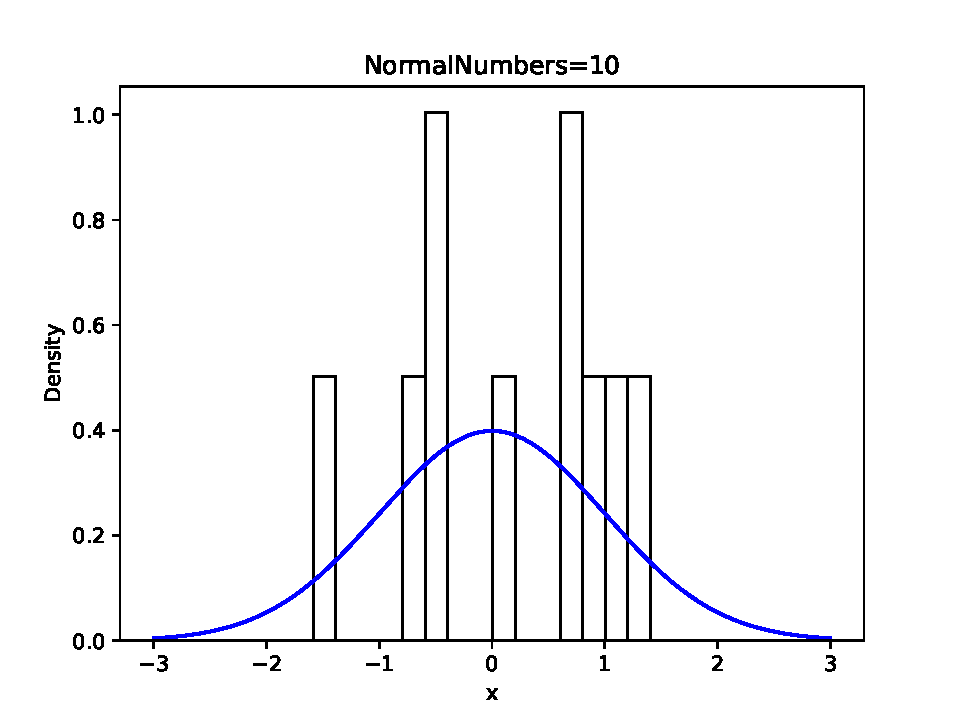
\includegraphics[scale=0.33]{normal_hist_10.pdf}
		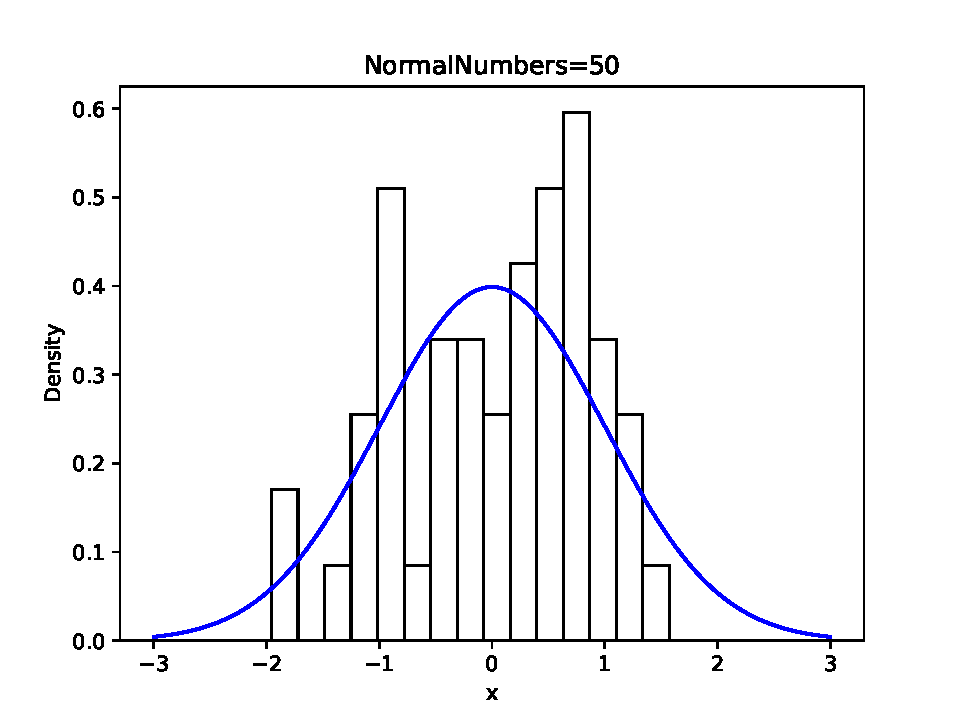
\includegraphics[scale=0.33]{normal_hist_50.pdf}
		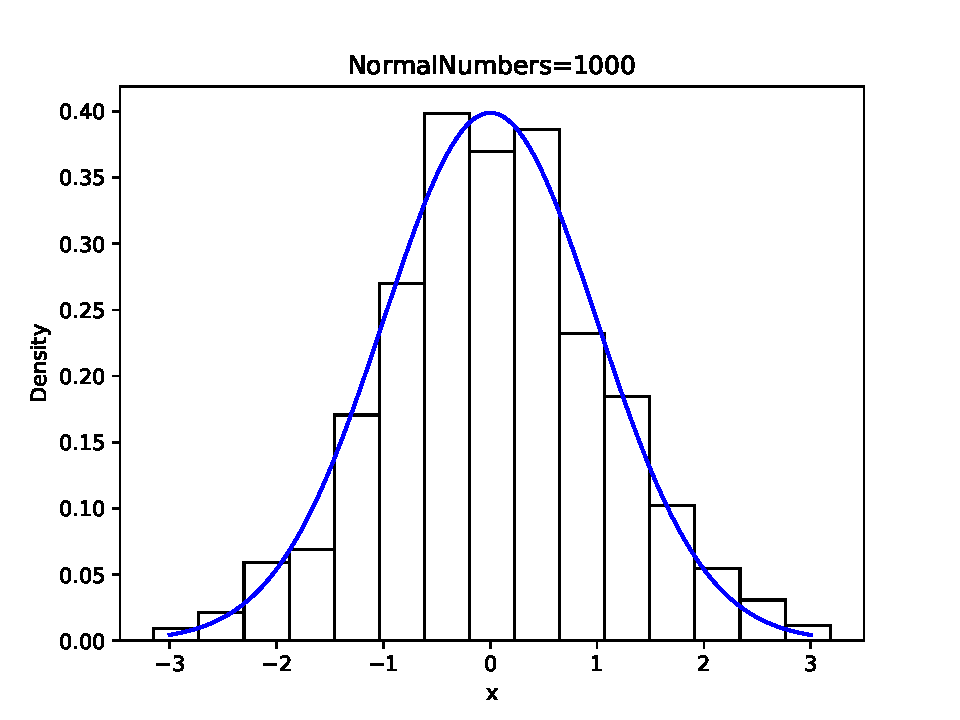
\includegraphics[scale=0.33]{normal_hist_1000.pdf}
	\end{tabular}
	\caption{Нормальное распределение}
\end{figure}

\begin{figure}[H]
	\begin{tabular}{ccc}
		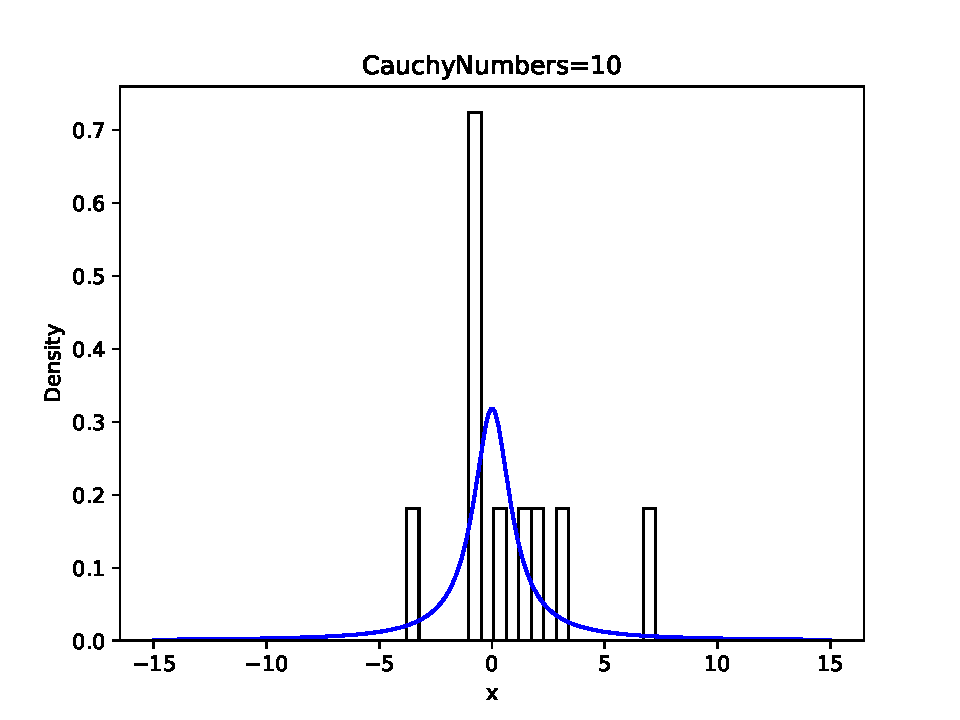
\includegraphics[scale=0.33]{cauchy_hist_10.pdf}
		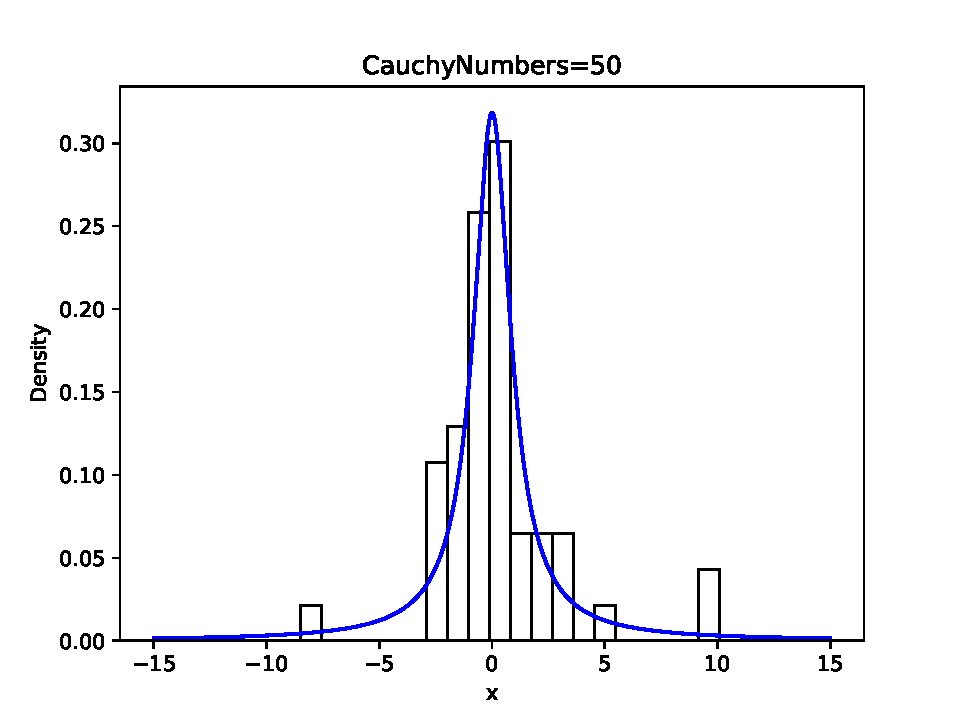
\includegraphics[scale=0.33]{cauchy_hist_50.pdf}
		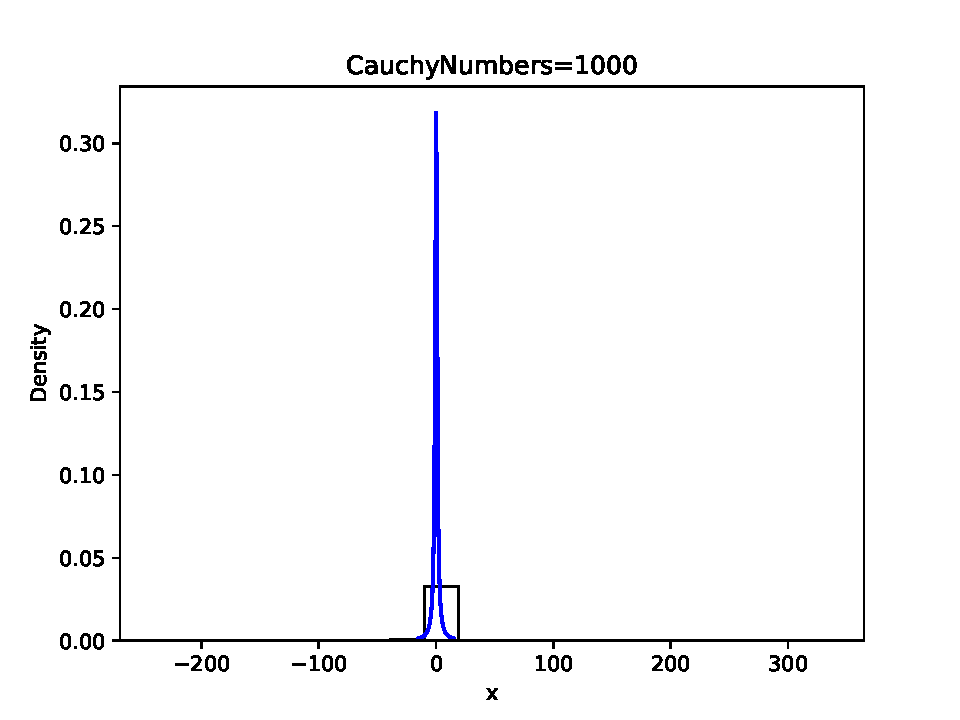
\includegraphics[scale=0.33]{cauchy_hist_1000.pdf}
	\end{tabular}
	\caption{Распределение Коши}
\end{figure}

\begin{figure}[H]
	\begin{tabular}{ccc}
		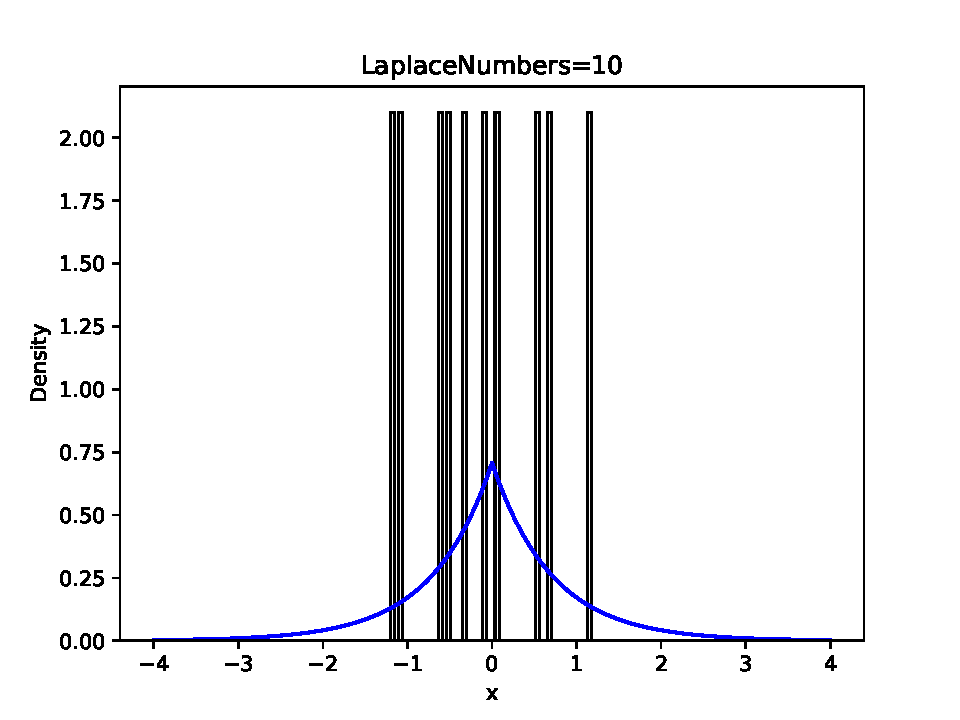
\includegraphics[scale=0.33]{laplace_hist_10.pdf}
		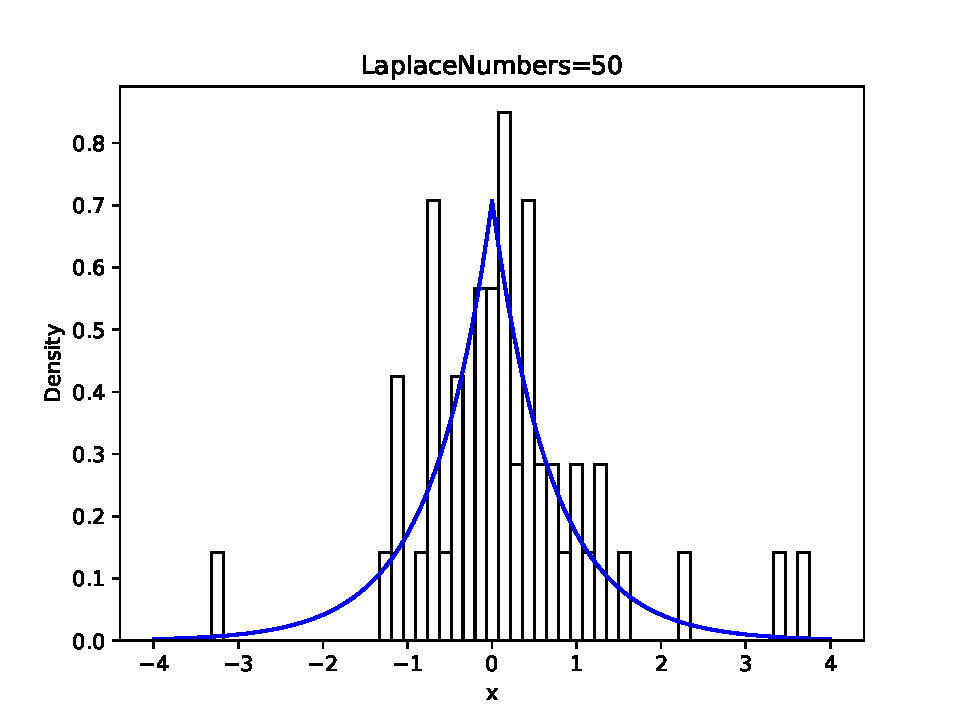
\includegraphics[scale=0.33]{laplace_hist_50.pdf}
		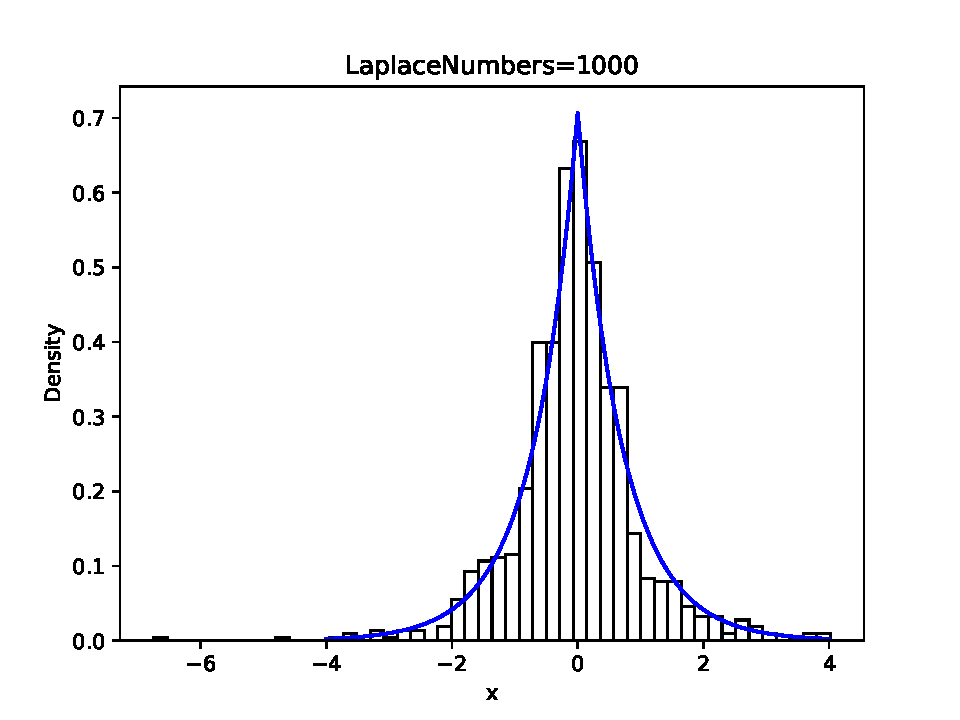
\includegraphics[scale=0.33]{laplace_hist_1000.pdf}
	\end{tabular}
	\caption{Распределение Лапласа}
\end{figure}

\begin{figure}[H]
	\begin{tabular}{ccc}
		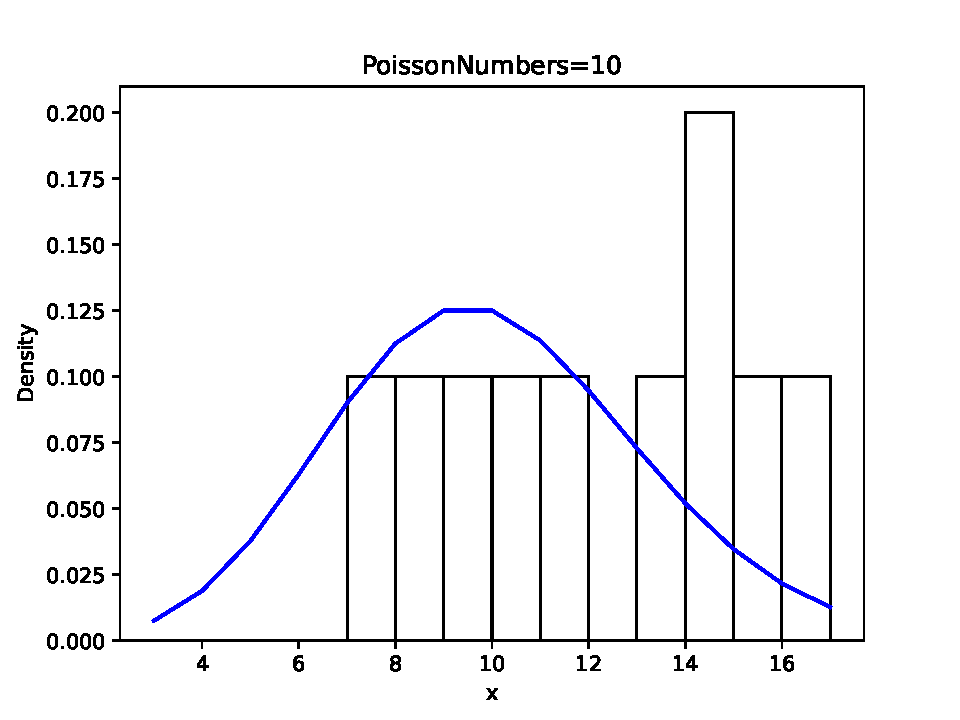
\includegraphics[scale=0.33]{poisson_hist_10.pdf}
		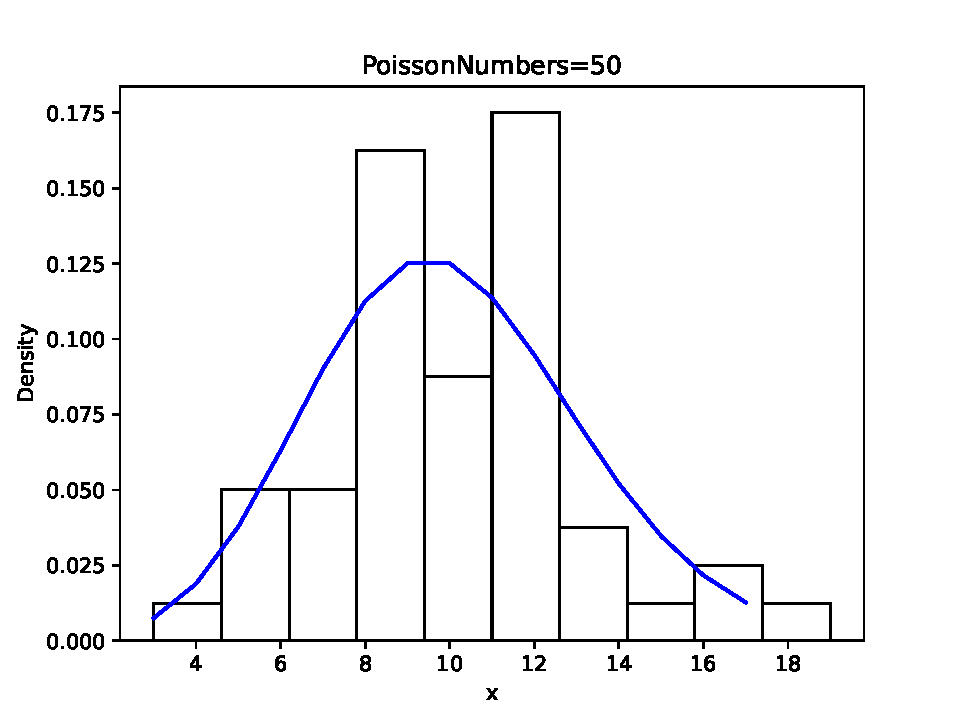
\includegraphics[scale=0.33]{poisson_hist_50.pdf}
		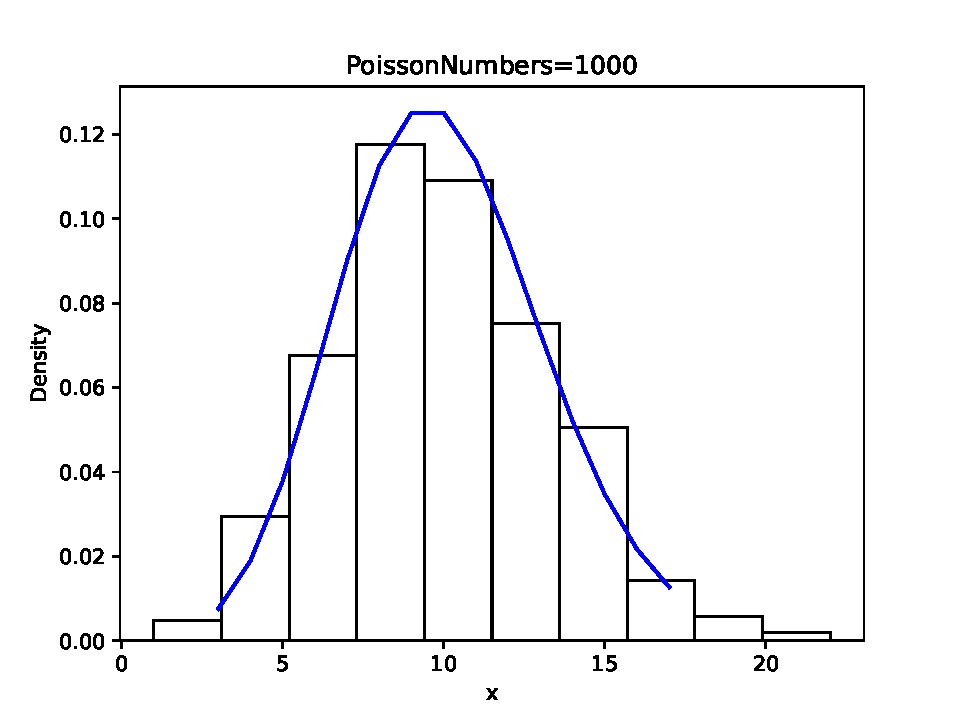
\includegraphics[scale=0.33]{poisson_hist_1000.pdf}
	\end{tabular}
	\caption{Распределение Пуассона}
\end{figure}


\begin{figure}[H]
	\begin{tabular}{ccc}
		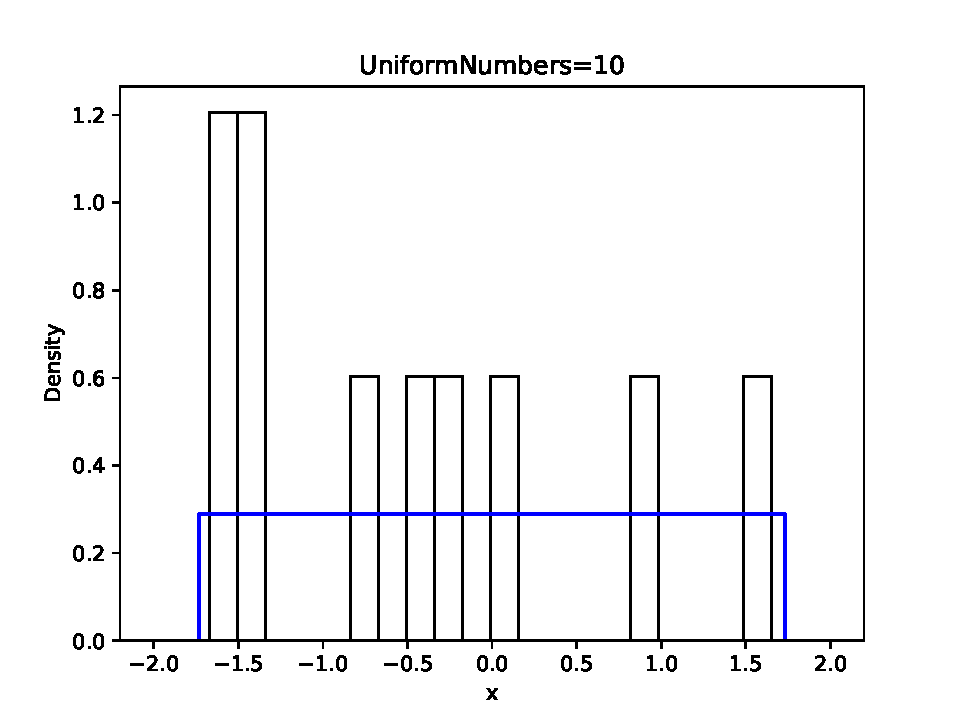
\includegraphics[scale=0.33]{uniform_hist_10.pdf}
		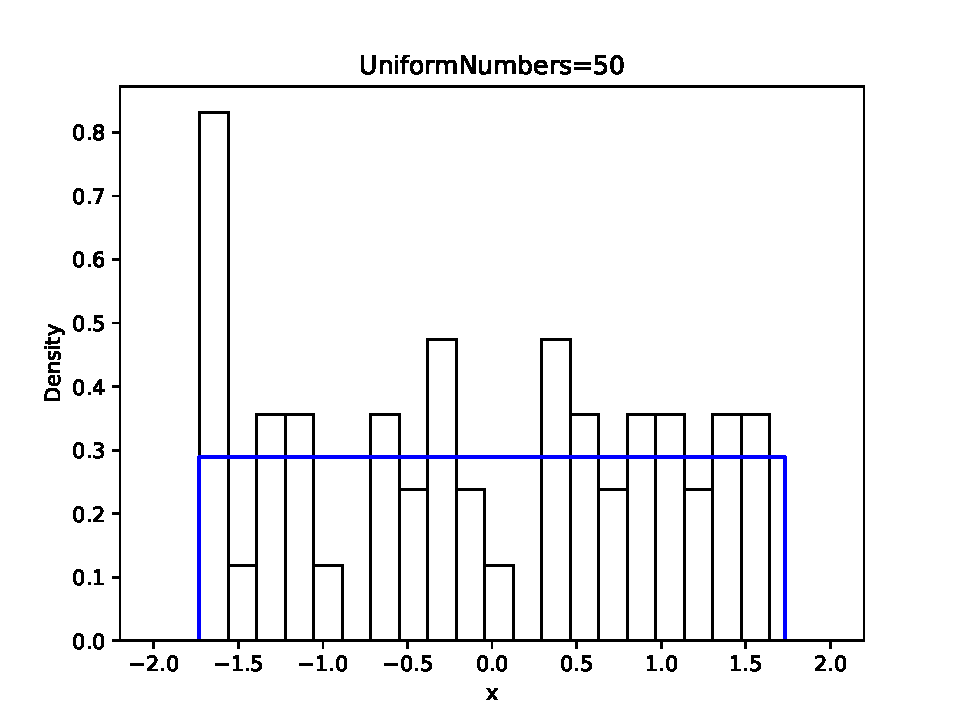
\includegraphics[scale=0.33]{uniform_hist_50.pdf}
		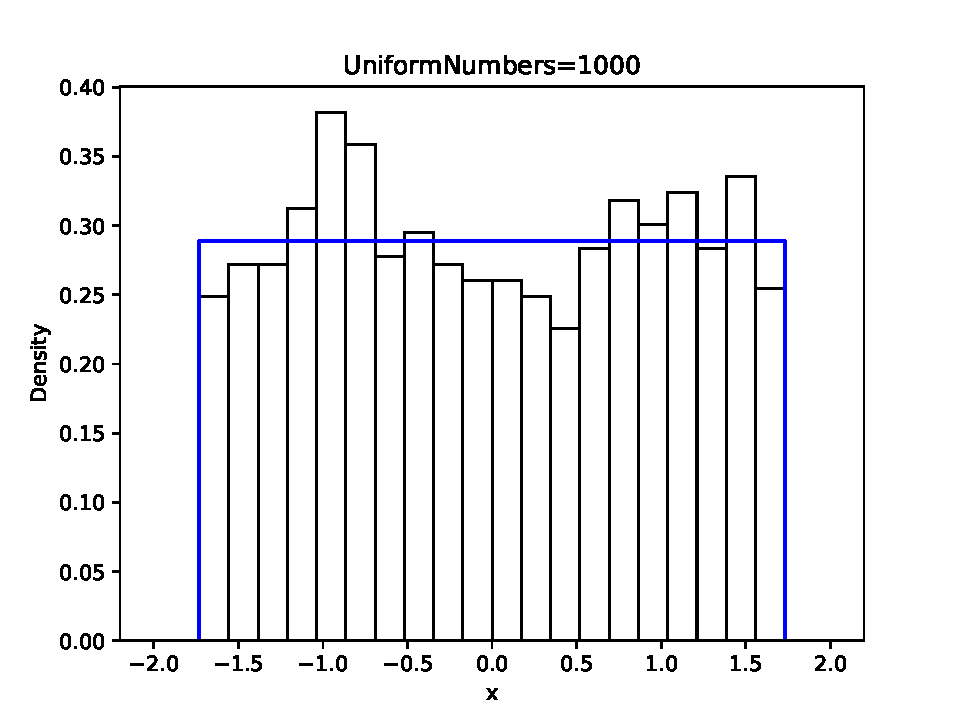
\includegraphics[scale=0.33]{uniform_hist_1000.pdf}
	\end{tabular}
	\caption{Равномерное распределение}
\end{figure}


\subsection{Характеристики положения и рассеяния}


 

\begin{table}[H]
	\begin{center}
		\begin{tabular}{|c||c|c|c|c|c|}
			\hline
			Normal n=10 & $\overline{x} $ & $med\:x$ & $z_{R}$ & $z_{Q}$ & $z_{tr}$ \\
			\hline\hline
			$E(z)$ & 0.00369 & 0.00140 & 0.00253 & 0.00218 & 0.00621 \\
			\hline
			$D(z)$ & 0.09933 & 0.13162 & 0.18904 & 0.12373 & 0.11933 \\
			\hline\hline
			Normal n=100 & $\overline{x} $ & $med\:x$ & $z_{R}$ & $z_{Q}$ & $z_{tr}$ \\
			\hline\hline
			$E(z)$ & -0.00061 & 0.00180 & 0.00675 & -0.01403 & -0.00010 \\
			\hline
			$D(z)$ & 0.00950 & 0.01575&  0.08953& 0.01197 & 0.01167  \\
			\hline\hline
			Normal n=1000 & $\overline{x} $ & $med\:x$ & $z_{R}$ & $z_{Q}$ & $z_{tr}$ \\
			\hline\hline
			$E(z)$ & -2.21952 & -0.00053 & -0.01664 & -0.00134 &   -0.00042 \\
			\hline
			$D(z)$ & 0.00101  & 0.00164 & 0.06311  &0.00124  & 0.00122 \\
			\hline
		\end{tabular}
	\end{center}
	\caption{Характеристики положения и рассеяния нормального распределения}
\end{table} 

\begin{table}[H]
	\begin{center}
		\begin{tabular}{|c||c|c|c|c|c|}
			\hline
			Cauchy n=10 & $\overline{x} $ & $med\:x$ & $z_{R}$ & $z_{Q}$ & $z_{tr}$ \\
			\hline\hline
			$E(z)$ & 0.60631 & -0.01793& 3.07935 & 0.00118 & -0.02171 \\
			\hline
			$D(z)$ & 3825.12746 & 0.36398 & 95430.01133 & 1.47888 & 0.38230 \\
			\hline\hline
			Cauchy n=100 & $\overline{x} $ & $med\:x$ & $z_{R}$ & $z_{Q}$ & $z_{tr}$ \\
			\hline\hline
			$E(z)$ & 0.68621 & -0.00218 & 33.379 & -0.02695 & 0.00145 \\
			\hline
			$D(z)$ &415.87354  &0.02449 & 1025245.02557 & 0.05200 &  0.02604\\
			\hline\hline
			Cauchy n=1000 & $\overline{x} $ & $med\:x$ & $z_{R}$ & $z_{Q}$ & $z_{tr}$ \\
			\hline\hline
			$E(z)$ & 0.02740 &-0.00038 & -5.55196 & -0.00173 & 7.45726 \\
			\hline
			$D(z)$ & 118.83309 &0.00243 & 28306188.93642 & 0.00501 &0.00252  \\
			\hline
		\end{tabular}
	\end{center}
	\caption{Характеристики положения и рассеяния распределения Коши}
\end{table}

\begin{table}[H]
	\begin{center}
		\begin{tabular}{|c||c|c|c|c|c|}
			\hline
			Laplace n=10 & $\overline{x} $ & $med\:x$ & $z_{R}$ & $z_{Q}$ & $z_{tr}$ \\
			\hline\hline
			$E(z)$ & 0.01279 &0.00579 & 0.02646 & 0.01273 & 0.00412 \\
			\hline
			$D(z)$ & 0.09453 &  0.07397 &  0.40262 &0.09303  &  0.06910 \\
			\hline\hline
			Laplace n=100 & $\overline{x} $ & $med\:x$ & $z_{R}$ & $z_{Q}$ & $z_{tr}$ \\
			\hline\hline
			$E(z)$ &0.00358  & 0.00157&0.00132  & -0.01101 & 0.00213 \\
			\hline
			$D(z)$ & 0.00990 &0.00523 & 0.42664 & 0.00966 & 0.00588 \\
			\hline\hline
			Laplace n=1000 & $\overline{x} $ & $med\:x$ & $z_{R}$ & $z_{Q}$ & $z_{tr}$ \\
			\hline\hline
			$E(z)$ & -0.00036 & 1.53039 & -0.01446 & -0.00114 & 0.00018 \\
			\hline
			$D(z)$ & 0.00102 &0.00050 & 0.41539 & 0.00096 & 0.00058  \\
			\hline
		\end{tabular}
	\end{center}
	\caption{Характеристики положения и рассеяния распределения Лапласа}
\end{table} 

\begin{table}[H]
	\begin{center}
		\begin{tabular}{|c||c|c|c|c|c|}
			\hline
			Poisson n=10 & $\overline{x} $ & $med\:x$ & $z_{R}$ & $z_{Q}$ & $z_{tr}$ \\
			\hline\hline
			$E(z)$ & 9.97609 &9.8235 & 10.2955 & 9.9105 &  9.8415  \\
			\hline
			$D(z)$ &0.97231  &1.37659 &1.79642 & 1.22023 & 1.21450 \\
			\hline\hline
			Poisson n=100 & $\overline{x} $ & $med\:x$ & $z_{R}$ & $z_{Q}$ & $z_{tr}$ \\
			\hline\hline
			$E(z)$ & 9.98505 & 9.836 & 10.9405  & 9.8475 & 9.84008 \\
			\hline
			$D(z)$ & 0.10400 & 0.22110 & 0.99120  & 0.16499 & 0.12406 \\
			\hline\hline
			Poisson n=1000 & $\overline{x} $ & $med\:x$ & $z_{R}$ & $z_{Q}$ & $z_{tr}$ \\
			\hline\hline
			$E(z)$ & 9.99791 & 9.9965 & 11.639 & 9.992  & 9.85761 \\
			\hline
			$D(z)$ &  0.00964 & 0.00323 & 0.61767 & 0.00443 & 0.01066 \\
			\hline
		\end{tabular}
	\end{center}
	\caption{Характеристики положения и рассеяния распределения Пуассона}
\end{table} 

\begin{table}[H]
	\begin{center}
		\begin{tabular}{|c||c|c|c|c|c|}
			\hline
			Uniform n=10 & $\overline{x} $ & $med\:x$ & $z_{R}$ & $z_{Q}$ & $z_{tr}$ \\
			\hline\hline
			$E(z)$ & 0.00336 &0.00843 & 0.00505 & -0.00111 & 0.00502 \\
			\hline
			$D(z)$ & 0.10159  & 0.22721 & 0.04560 & 0.14254 & 0.19700 \\
			\hline\hline
			Uniform n=100 & $\overline{x} $ & $med\:x$ & $z_{R}$ & $z_{Q}$ & $z_{tr}$ \\
			\hline\hline
			$E(z)$ & 0.00098 & 0.00587 & 0.00060 & -0.01393 &  0.00199\\
			\hline
			$D(z)$ & 0.01036 & 0.03018 & 0.00057 & 0.01545 & 0.02068  \\
			\hline\hline
			Uniform n=1000 & $\overline{x} $ & $med\:x$ & $z_{R}$ & $z_{Q}$ & $z_{tr}$ \\
			\hline\hline
			$E(z)$ & -0.00111 &-0.00171 & -0.00003 & -0.00240 & -0.00139  \\
			\hline
			$D(z)$ & 0.00100 & 0.00288 & 5.99778 & 0.00154 & 0.00198 \\
			\hline
		\end{tabular}
	\end{center}
	\caption{Характеристики положения и рассеяния равномерного распределения}
\end{table} 